\documentclass[12pt]{scrartcl}
    \usepackage[a4paper,margin=2.5cm]{geometry}
    \usepackage[hidelinks]{hyperref}
    \usepackage[utf8]{inputenc}
    \usepackage[T1]{fontenc}
    \usepackage{fancyhdr}
    \usepackage{graphicx}
    \usepackage{xcolor}
    \usepackage{listings}
    \usepackage{amsmath}
    \usepackage{amsfonts}
    \usepackage{amssymb}
    \usepackage{booktabs}
    \usepackage{longtable}
    \usepackage{enumitem}
    \usepackage{framed}
    \usepackage{setspace}

    % for the landscape diagram page
    \usepackage{pdflscape}

    % for the TikZ diagram
    \usepackage{tikz}
    \usetikzlibrary{positioning, arrows.meta, shapes, fit, calc}

    % Variablen definieren
    \newcommand{\faculty}{Faculty Applied Information Technology}
    \newcommand{\studies}{Bachelor of Cyber-Security}
    \newcommand{\thesistitleDE}{Damn Vulnerable Drone Supply Chain Compromise - Project Docs}
    \newcommand{\submissiondate}{17.\ Juli 2025}
    \newcommand{\supervisor}{Prof.\ Dr.\ Michael Heigl}

    \definecolor{codegreen}{rgb}{0,0.6,0}
    \definecolor{codegray}{rgb}{0.5,0.5,0.5}
    \definecolor{codepurple}{rgb}{0.58,0,0.82}
    \definecolor{backcolour}{rgb}{0.95,0.95,0.92}
    \definecolor{alertred}{rgb}{0.8,0.1,0.1}
    \definecolor{flagblue}{rgb}{0.1,0.3,0.8}
    \definecolor{hintgreen}{rgb}{0.1,0.7,0.2}
    \definecolor{warningorange}{rgb}{0.9,0.5,0.1}

    \lstdefinestyle{mystyle}{
        backgroundcolor=\color{backcolour},   
        commentstyle=\color{codegreen},
        keywordstyle=\color{magenta},
        numberstyle=\tiny\color{codegray},
        stringstyle=\color{codepurple},
        basicstyle=\ttfamily\footnotesize,
        breakatwhitespace=false,         
        breaklines=true,                 
        captionpos=b,                    
        keepspaces=true,                 
        numbers=left,                    
        numbersep=5pt,                  
        showspaces=false,                
        showstringspaces=false,
        showtabs=false,                  
        tabsize=2
    }

    \lstset{style=mystyle}

    % Custom environments for different types of content
    \newenvironment{flagbox}{%
    \def\FrameCommand{\fboxsep=\FrameSep\colorbox{flagblue!20}}%
    \MakeFramed {\advance\hsize-\width \FrameRestore}}%
    {\endMakeFramed}

    \newenvironment{hintbox}{%
    \def\FrameCommand{\fboxsep=\FrameSep\colorbox{hintgreen!20}}%
    \MakeFramed {\advance\hsize-\width \FrameRestore}}%
    {\endMakeFramed}

    \newenvironment{warningbox}{%
    \def\FrameCommand{\fboxsep=\FrameSep\colorbox{warningorange!20}}%
    \MakeFramed {\advance\hsize-\width \FrameRestore}}%
    {\endMakeFramed}

    \newenvironment{storybox}{%
    \def\FrameCommand{\fboxsep=\FrameSep\colorbox{gray!10}}%
    \MakeFramed {\advance\hsize-\width \FrameRestore}}%
    {\endMakeFramed}

    % Custom environment for challenge boxes
    \newenvironment{challengebox}[1]{%
    \def\FrameCommand{\fboxsep=\FrameSep\colorbox{flagblue!10}}%
    \MakeFramed{\advance\hsize-\width \FrameRestore}
    \noindent\textbf{Challenge:} #1\\[0.5em]
    \vspace{0.5em}
    \begin{minipage}{0.95\linewidth}
    }{%
    \\[1em]
    \noindent\rule{\linewidth}{0.4pt}\\[2em] % Dedicated answer field
    \end{minipage}
    \endMakeFramed
    }

    \pagestyle{fancy}
    \fancyhf{}
    \rfoot{Page \thepage}

    \begin{document}

    \begin{titlepage}
    \begin{center}
        {\Large Technische Hochschule Deggendorf\\
        \faculty\par}
        \vspace{0.2cm}
        {\Large Studiengang \studies\\}
        \vspace{2\baselineskip}
        {\Huge\bfseries \thesistitleDE\par}
        \vspace{3\baselineskip}
    \end{center}

    \vfill

    \parbox[t]{0.4\textwidth}{
        \textbf{Vorgelegt von:}\\[0.5em]
        Christof Renner\\
        Matrikelnummer: 22301943\\
        Manuel Friedl\\
        Matrikelnummer: 1236626\\
        Felix Hahl\\
        Matrikelnummer:\\[1em]
        \\
        Am: \submissiondate\par
    }
    \hfill
    \parbox[t]{0.4\textwidth}{
        \textbf{Prüfungsleitung:}\\[0.5em]
        \supervisor
    }
    \end{titlepage}

    \cleardoublepage
    \tableofcontents
    \cleardoublepage

    \section{Einleitung und Projektübersicht}
    
    Dieses Dokument beschreibt die Entwicklung und technische Umsetzung des „Damn Vulnerable Drone Supply Chain Compromise" CTF-Projekts. Das Projekt wurde im Rahmen des Studiengangs Cyber-Security an der Technischen Hochschule Deggendorf entwickelt und dient als praktische Lernumgebung für Supply-Chain-Angriffe im Kontext von Drohnensystemen.

    \subsection{Zielsetzung}
    
    Das Hauptziel dieses Projekts bestand darin, eine realistische Simulationsumgebung zu schaffen, in der Studierende praxisnah die Konzepte und Techniken von Supply-Chain-Angriffen erlernen und anwenden können. Dabei wurden folgende spezifische Lernziele definiert:
    
    \begin{itemize}
        \item Verständnis der grundlegenden Architektur von Drohnensystemen
        \item Praktische Anwendung von Reconnaissance-Techniken in Linux-Umgebungen
        \item Identifikation und Ausnutzung von Schwachstellen in Build-Prozessen
        \item Implementierung von Supply-Chain-Angriffen zur Kompromittierung von Drohnensoftware
        \item Analyse der Angriffstechniken im Kontext des MITRE ATT\&CK-Frameworks
    \end{itemize}
    
    \subsection{Projektkontext}
    
    Das Projekt basiert auf dem Open-Source-Projekt „Damn Vulnerable Drone" von Nicholas Aleks, das eine virtuelle Drohnenumgebung für Sicherheitstests bietet. Für unsere Zwecke haben wir dieses Projekt erweitert und ein spezifisches CTF-Szenario entwickelt, das auf Supply-Chain-Angriffe fokussiert ist. Die Herausforderung besteht darin, durch Ausnutzung einer Sicherheitslücke im Entwicklungsprozess einer simulierten Drohnensoftwarefirma, eine Drohne zum Absturz zu bringen.

    \section{Technische Architektur}
    
    \subsection{Gesamtarchitektur}
    
    Die Simulationsumgebung wurde vollständig mit Docker-Containern realisiert, um eine konsistente und isolierte Lernumgebung zu gewährleisten. Die Hauptkomponenten des Systems sind:
    
    \begin{figure}[h]
    \centering
    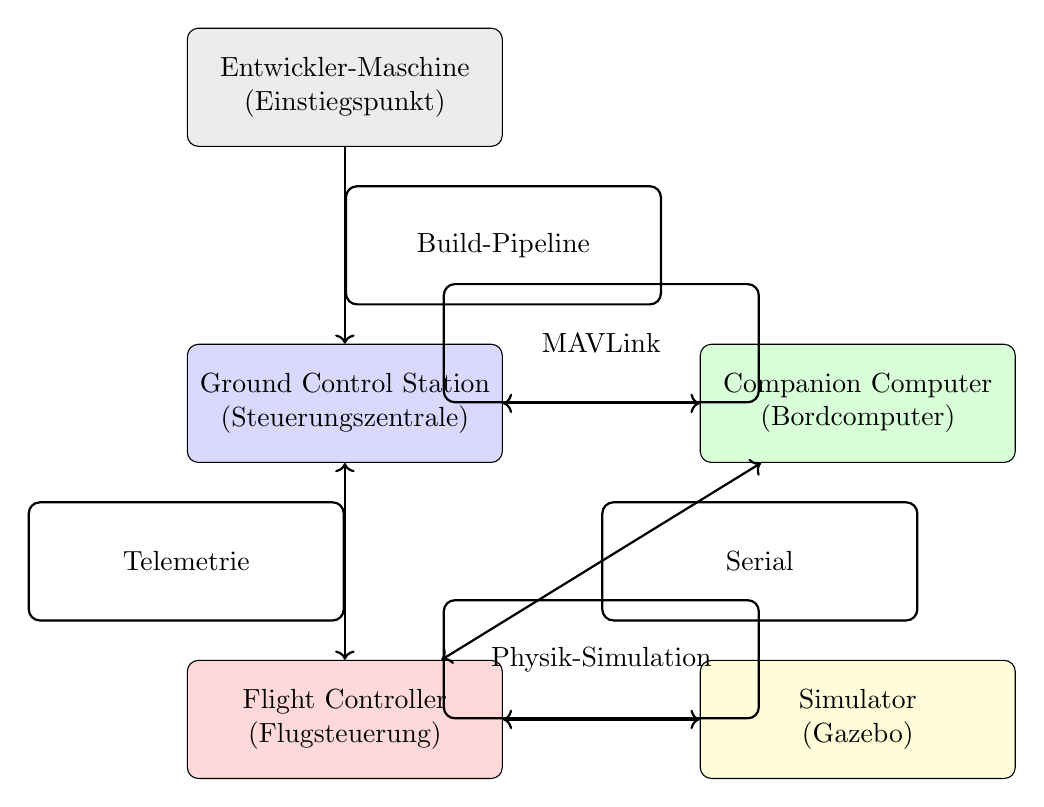
\begin{tikzpicture}[node distance=2.5cm, every node/.style={rectangle, rounded corners, draw, align=center, minimum width=4cm, minimum height=1.5cm}]
        % Container nodes
        \node[fill=gray!15] (dev) {Entwickler-Maschine\\(Einstiegspunkt)};
        \node[fill=blue!15, below=of dev] (gcs) {Ground Control Station\\(Steuerungszentrale)};
        \node[fill=green!15, right=of gcs] (companion) {Companion Computer\\(Bordcomputer)};
        \node[fill=red!15, below=of gcs] (flight) {Flight Controller\\(Flugsteuerung)};
        \node[fill=yellow!15, right=of flight] (simulator) {Simulator\\(Gazebo)};
        
        % Connections
        \draw[->, thick] (dev) -- node[right] {Build-Pipeline} (gcs);
        \draw[<->, thick] (gcs) -- node[above] {MAVLink} (companion);
        \draw[<->, thick] (gcs) -- node[left] {Telemetrie} (flight);
        \draw[<->, thick] (companion) -- node[right] {Serial} (flight);
        \draw[<->, thick] (flight) -- node[above] {Physik-Simulation} (simulator);
    \end{tikzpicture}
    \caption{Architektur der Simulationsumgebung}
    \end{figure}
    
    \subsection{Containerdetails}
    
    \begin{itemize}
        \item \textbf{Entwickler-Maschine:} Dient als Einstiegspunkt für die Teilnehmer und simuliert die Arbeitsumgebung eines Entwicklers bei einer Drohnensoftwarefirma. Enthält Entwicklungswerkzeuge und automatisierte Build-Skripte.
        
        \item \textbf{Ground Control Station (GCS):} Stellt die Bodenkontrollstation dar, von der aus die Drohne gesteuert wird. Implementiert das zu kompromittierende "Return-to-Land"-Modul.
        
        \item \textbf{Companion Computer:} Simuliert den Bordcomputer der Drohne, der für fortgeschrittene Funktionen wie Bildverarbeitung, Navigation und Kommunikation zuständig ist.
        
        \item \textbf{Flight Controller:} Repräsentiert die eigentliche Flugsteuerung der Drohne, basierend auf ArduPilot-Firmware, und verarbeitet die Steuerbefehle.
        
        \item \textbf{Simulator:} Gazebo-basierte 3D-Umgebung, die die physikalischen Eigenschaften der Drohne und ihre Interaktion mit der Umgebung simuliert.
    \end{itemize}
    
    \subsection{Netzwerkstruktur}
    
    Die Container sind in zwei Netzwerken organisiert:
    
    \begin{itemize}
        \item \textbf{Infrastrukturnetzwerk (10.13.0.0/24):} Verbindet alle Container miteinander und ermöglicht die grundlegende Kommunikation zwischen den Systemkomponenten.
        
        \item \textbf{Simuliertes WLAN (192.168.13.0/24):} Simuliert die drahtlose Verbindung zwischen der Ground Control Station und dem Companion Computer. Dieses Netzwerk wird virtuell über Container-Links implementiert.
    \end{itemize}
    
    \begin{figure}[h]
    \centering
    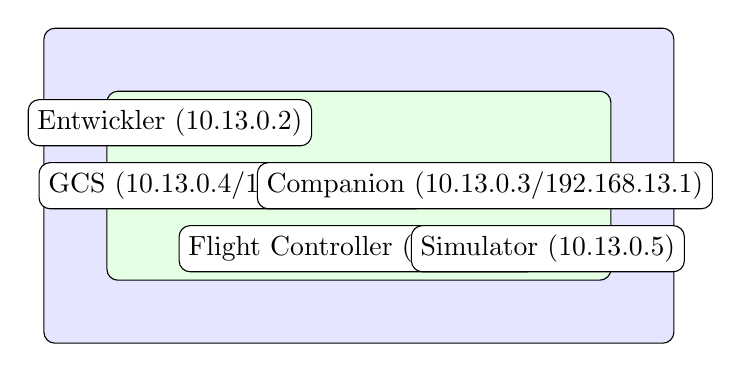
\begin{tikzpicture}[scale=0.8, node distance=2cm]
        % Draw networks
        \draw[rounded corners, fill=blue!10] (0,0) rectangle (10,5) node[pos=.5] {Infrastrukturnetzwerk (10.13.0.0/24)};
        \draw[rounded corners, fill=green!10] (1,1) rectangle (9,4) node[pos=.5] {Simuliertes WLAN (192.168.13.0/24)};
        
        % Draw network components
        \node[draw, fill=white, rounded corners] (dev) at (2,3.5) {Entwickler (10.13.0.2)};
        \node[draw, fill=white, rounded corners] (gcs) at (3,2.5) {GCS (10.13.0.4/192.168.13.14)};
        \node[draw, fill=white, rounded corners] (comp) at (7,2.5) {Companion (10.13.0.3/192.168.13.1)};
        \node[draw, fill=white, rounded corners] (flight) at (5,1.5) {Flight Controller (10.13.0.2)};
        \node[draw, fill=white, rounded corners] (sim) at (8,1.5) {Simulator (10.13.0.5)};
    \end{tikzpicture}
    \caption{Netzwerkstruktur der Simulationsumgebung}
    \end{figure}

    \section{Entwicklungsprozess}
    
    \subsection{Konzeption und Planung}
    
    Die Entwicklung des CTF-Szenarios begann mit einer detaillierten Konzeptphase. Zuerst analysierten wir die ursprüngliche Damn Vulnerable Drone-Plattform, um ein Verständnis für ihre Funktionsweise und Möglichkeiten zu entwickeln. Anschließend definierten wir das Szenario eines Supply-Chain-Angriffs, bei dem ein Angreifer Zugriff auf die Entwicklungsumgebung einer Drohnensoftwarefirma erhält und versucht, schädlichen Code in den Build-Prozess einzuschleusen.
    
    Wir legten folgende Designprinzipien fest:
    
    \begin{itemize}
        \item \textbf{Realismus:} Das Szenario sollte realistische Schwachstellen widerspiegeln, die in tatsächlichen Entwicklungsumgebungen vorkommen könnten.
        
        \item \textbf{Lernwert:} Jeder Schritt der Challenge sollte wichtige Sicherheitskonzepte vermitteln.
        
        \item \textbf{Zugänglichkeit:} Die Challenge sollte für Studierende mit grundlegenden Linux-Kenntnissen lösbar sein.
        
        \item \textbf{Skalierbarkeit:} Die Umgebung sollte auf verschiedenen Systemen lauffähig sein, mit minimalen Anforderungen.
    \end{itemize}
    
    \subsection{Technische Implementierung}
    
    Die Implementierung erfolgte in mehreren Phasen:
    
    \begin{enumerate}
        \item \textbf{Container-Setup:} Erstellung der Docker-Container für die verschiedenen Komponenten des Systems. Wir verwendeten Alpine Linux als Basis für die meisten Container, um die Größe zu minimieren.
        
        \item \textbf{Integration der Drohnensimulation:} Konfiguration von ArduPilot SITL (Software-in-the-Loop) und Gazebo für die realistische Simulation des Drohnenverhaltens.
        
        \item \textbf{Implementierung der Build-Pipeline:} Entwicklung der automatisierten Build- und Deployment-Prozesse, die als Angriffsziel dienen. Dies umfasste die Erstellung von Cron-Jobs und Bash-Skripten.
        
        \item \textbf{Implementierung der Schwachstellen:} Gezielte Integration von Sicherheitslücken, insbesondere im Zusammenhang mit Berechtigungen und unsicheren Automatisierungsprozessen.
        
        \item \textbf{Entwicklung des Web-Interfaces:} Erstellung einer benutzerfreundlichen Weboberfläche zur Steuerung der Simulation und Visualisierung des Drohnenverhaltens.
        
        \item \textbf{Dokumentation und Walkthrough:} Erstellung detaillierter Anleitungen sowohl für die Setup-Phase als auch für die Lösung der Challenge.
    \end{enumerate}
    
    \subsection{Sicherheitslücken und Angriffspfad}
    
    Der Hauptangriffspfad der Challenge beinhaltet folgende Schritte:
    
    \begin{enumerate}
        \item \textbf{Initiale Zugriff:} Teilnehmer erhalten Zugang zur Entwickler-Maschine mit den Anmeldedaten eines Junior-Entwicklers (developer:dev123).
        
        \item \textbf{Reconnaissance:} Erkundung der Umgebung, um Systemstrukturen und potenzielle Angriffspunkte zu identifizieren.
        
        \item \textbf{Entdeckung der Build-Pipeline:} Identifikation des automatisierten Build-Prozesses und seiner Komponenten.
        
        \item \textbf{Ausnutzung von Cron-Jobs:} Analyse der als Root ausgeführten Cron-Jobs und Identifikation der Build-Update-Skripte.
        
        \item \textbf{Code-Injektion:} Modifikation des Quellcodes oder der Docker-Dateien, um schädlichen Code in den Build-Prozess einzuschleusen.
        
        \item \textbf{Persistence:} Warten auf die automatische Ausführung des Build-Prozesses und Deployment des modifizierten Codes.
        
        \item \textbf{Impact:} Auslösen des "Return-to-Land"-Befehls, der nun durch den injizierten Code die Drohne zum Absturz bringt.
    \end{enumerate}
    
    Diese Schritte entsprechen mehreren Taktiken des MITRE ATT\&CK-Frameworks, darunter Initial Access, Discovery, Persistence, Privilege Escalation, Defense Evasion und Impact.

    \section{Arbeitsaufteilung}
    
    Die Entwicklung des Projekts wurde auf mehrere Teammitglieder aufgeteilt, wobei jedes Mitglied spezifische Verantwortungsbereiche übernahm. Die folgende Tabelle zeigt die detaillierte Arbeitsaufteilung:
    
    \begin{longtable}{|p{3cm}|p{5cm}|p{6cm}|}
    \hline
    \textbf{Teammitglied} & \textbf{Hauptverantwortlichkeiten} & \textbf{Spezifische Aufgaben} \\
    \hline
    \endhead
    
    Christof Renner & Technische Architektur \& Docker-Integration & 
    \begin{itemize}
      \item Entwicklung der Container-Architektur
      \item Konfiguration der Netzwerkstruktur
      \item Integration der Build-Pipeline
      \item Implementation der Schwachstellen
    \end{itemize} \\
    \hline
    
    Manuel Friedl & Drohnensimulation \& Web-Interface & 
    \begin{itemize}
      \item Konfiguration von ArduPilot SITL
      \item Integration von Gazebo
      \item Entwicklung des MAVLink-Kommunikationssystems
      \item Erstellung der Simulationsszenarien
    \end{itemize} \\
    \hline
    
    Felix Hahl & Dokumentation \& Testing & 
    \begin{itemize}
      \item Erstellung der technischen Dokumentation
      \item Entwicklung des Walkthroughs
      \item Qualitätssicherung und Testing
      \item Erstellung von Lernmaterialien
    \end{itemize} \\
    \hline
    \end{longtable}
    
    Die Arbeitsverteilung basierte auf den individuellen Stärken und Interessen der Teammitglieder, wobei regelmäßige Abstimmungen und gemeinsame Review-Sessions sicherstellten, dass alle Komponenten nahtlos zusammenarbeiten. Die Entwicklung erfolgte in einem agilen Prozess mit wöchentlichen Sprints und kontinuierlicher Integration der Teilkomponenten.

    \section{Technische Herausforderungen und Lösungen}
    
    \subsection{Blockers: Schwierigkeiten mit virtuellen Maschinen}
    
    Während der Entwicklung des Projekts stießen wir auf mehrere signifikante technische Herausforderungen, insbesondere im Zusammenhang mit der Ausführung in virtuellen Maschinen:
    
    \begin{warningbox}
    \textbf{Hauptproblem: Grafikbeschleunigung in VMs}
    
    Eine der größten Herausforderungen war die fehlende Grafikbeschleunigung in virtuellen Maschinen. Der Gazebo-Simulator erfordert OpenGL-Unterstützung für die 3D-Visualisierung der Drohne und ihrer Umgebung. In virtuellen Maschinen ohne durchgereichte GPU war die Performance extrem eingeschränkt oder die Simulation funktionierte gar nicht.
    \end{warningbox}
    
    \subsubsection{Spezifische VM-bezogene Probleme}
    
    \begin{itemize}
        \item \textbf{Grafikprobleme:} Die 3D-Darstellung in Gazebo benötigt OpenGL-Unterstützung, die in Standard-VMs oft nicht verfügbar ist.
        
        \item \textbf{Performance-Engpässe:} Die Simulation der Drohnenphysik und der 3D-Umgebung ist rechenintensiv und führte in VMs zu erheblichen Leistungseinbußen.
        
        \item \textbf{Netzwerk-Isolation:} Die komplexe Netzwerkstruktur mit Docker-Containern und virtuellen Netzwerken führte in verschachtelten Virtualisierungsumgebungen zu Konnektivitätsproblemen.
        
        \item \textbf{Instabilität:} In virtuellen Umgebungen kam es häufiger zu Abstürzen der Simulation, insbesondere bei längerer Laufzeit.
    \end{itemize}
    
    \subsection{Lösungsansätze}
    
    Um diese Herausforderungen zu bewältigen, haben wir verschiedene Lösungsansätze entwickelt:
    
    \begin{itemize}
        \item \textbf{Headless-Modus:} Implementierung eines "Headless"-Modus für Gazebo, der ohne grafische Oberfläche arbeitet und die 3D-Visualisierung auf ein Minimum reduziert.
        
        \item \textbf{Ressourcen-Optimierung:} Anpassung der Container-Konfigurationen zur Minimierung des Ressourcenverbrauchs, insbesondere durch Verwendung leichtgewichtiger Linux-Distributionen.
        
        \item \textbf{Performance-Monitoring:} Entwicklung von Skripten zur Überwachung der Systemleistung und automatischen Anpassung der Simulationsparameter.
        
        \item \textbf{Alternative Visualisierung:} Implementierung einer webbasierten Visualisierung, die weniger ressourcenintensiv ist als die native Gazebo-Darstellung.
        
        \item \textbf{Dokumentation von Mindestanforderungen:} Klare Definition der Systemvoraussetzungen und Bereitstellung von Installationsanleitungen für verschiedene Host-Systeme.
    \end{itemize}
    
    \begin{figure}[h]
    \centering
    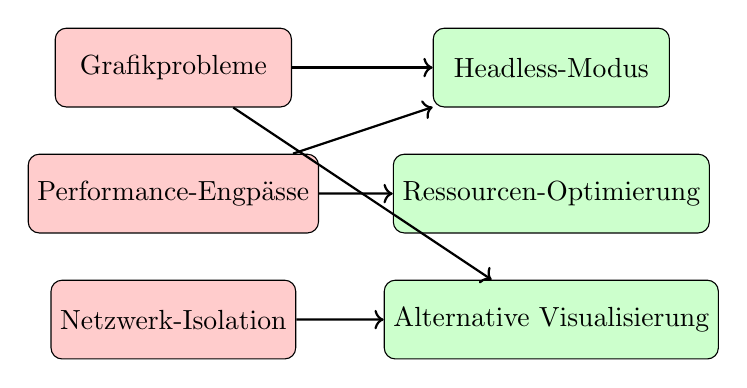
\begin{tikzpicture}[scale=0.8, every node/.style={rectangle, rounded corners, draw, minimum width=3cm, minimum height=1cm}]
        % Problem nodes
        \node[fill=red!20] (problem1) at (0,0) {Grafikprobleme};
        \node[fill=red!20] (problem2) at (0,-2) {Performance-Engpässe};
        \node[fill=red!20] (problem3) at (0,-4) {Netzwerk-Isolation};
        
        % Solution nodes
        \node[fill=green!20] (solution1) at (6,0) {Headless-Modus};
        \node[fill=green!20] (solution2) at (6,-2) {Ressourcen-Optimierung};
        \node[fill=green!20] (solution3) at (6,-4) {Alternative Visualisierung};
        
        % Arrows
        \draw[->, thick] (problem1) -- (solution1);
        \draw[->, thick] (problem2) -- (solution2);
        \draw[->, thick] (problem3) -- (solution3);
        \draw[->, thick] (problem1) -- (solution3);
        \draw[->, thick] (problem2) -- (solution1);
    \end{tikzpicture}
    \caption{Probleme und Lösungsansätze bei VM-Herausforderungen}
    \end{figure}
    
    \subsection{Performance-Optimierung}
    
    Ein weiterer kritischer Aspekt war die Performance-Optimierung, insbesondere für Systeme mit begrenzten Ressourcen:
    
    \begin{itemize}
        \item \textbf{Container-Konfiguration:} Feinabstimmung der Docker-Container-Ressourcen (CPU, Speicher) für optimale Performance.
        
        \item \textbf{Simulation-Vereinfachung:} Reduzierung der Komplexität des Gazebo-Modells und der Physik-Simulation.
        
        \item \textbf{Parallelisierung:} Verteilung rechenintensiver Prozesse auf mehrere Container und Optimierung der Kommunikation zwischen ihnen.
        
        \item \textbf{Caching-Strategien:} Implementierung von Caching-Mechanismen für häufig verwendete Daten und Simulationsergebnisse.
    \end{itemize}
    
    \begin{table}[h]
    \centering
    \begin{tabular}{|l|l|l|}
    \hline
    \textbf{Performance-Maßnahme} & \textbf{Vor Optimierung} & \textbf{Nach Optimierung} \\
    \hline
    CPU-Auslastung & 95-100\% & 60-75\% \\
    \hline
    RAM-Verbrauch & 8+ GB & 4-6 GB \\
    \hline
    Simulationsgeschwindigkeit & 0.5x Echtzeit & 1.0x Echtzeit \\
    \hline
    Container-Startzeit & 90+ Sekunden & 45-60 Sekunden \\
    \hline
    \end{tabular}
    \caption{Performance-Verbesserungen durch Optimierungsmaßnahmen}
    \end{table}

    \section{Testergebnisse und Evaluation}
    
    \subsection{Testmethodik}
    
    Um die Funktionalität und Benutzererfahrung der CTF-Challenge zu evaluieren, führten wir verschiedene Tests durch:
    
    \begin{itemize}
        \item \textbf{Funktionalitätstests:} Überprüfung aller Komponenten und deren Zusammenspiel.
        
        \item \textbf{Usability-Tests:} Bewertung der Benutzerfreundlichkeit und Zugänglichkeit der Challenge.
        
        \item \textbf{Performance-Tests:} Messung der Systemleistung unter verschiedenen Bedingungen.
        
        \item \textbf{Kompatibilitätstests:} Überprüfung der Lauffähigkeit auf verschiedenen Host-Systemen.
    \end{itemize}
    
    \subsection{Feedback und Iterationen}
    
    Auf Basis des Teilnehmerfeedbacks wurden mehrere Verbesserungen vorgenommen:
    
    \begin{itemize}
        \item \textbf{Verbesserte Dokumentation:} Ergänzung der Anleitungen mit mehr Hintergrundinformationen und Konzepterklärungen.
        
        \item \textbf{Performance-Optimierungen:} Weitere Maßnahmen zur Reduzierung des Ressourcenverbrauchs für bessere Kompatibilität.
        
        \item \textbf{Alternative Lösungswege:} Implementierung mehrerer möglicher Angriffspfade, um unterschiedliche Lernerfahrungen zu ermöglichen.
        
        \item \textbf{Checkpoints:} Einführung von Zwischenzielen, um den Fortschritt besser verfolgen zu können.
    \end{itemize}

    \section{Fazit und Ausblick}
    
    \subsection{Projektergebnisse}
    
    Das Damn Vulnerable Drone Supply Chain Compromise CTF-Projekt wurde erfolgreich entwickelt und implementiert. Es bietet eine realistische und lehrreiche Umgebung, in der Studierende praktische Erfahrungen mit Supply-Chain-Angriffen sammeln können. Die wichtigsten Errungenschaften des Projekts sind:
    
    \begin{itemize}
        \item Eine vollständig funktionsfähige Drohnensimulationsumgebung, die realistische Angriffszenarien ermöglicht.
        
        \item Ein strukturierter Lernpfad mit klaren Lernzielen und praktischen Übungen.
        
        \item Eine detaillierte Dokumentation, die sowohl den Aufbau der Umgebung als auch die Lösungswege erläutert.
        
        \item Eine optimierte Containerarchitektur, die auf verschiedenen Systemen lauffähig ist.
    \end{itemize}
    
    \subsection{Lehren aus dem Projekt}
    
    Während der Entwicklung haben wir wichtige Erkenntnisse gewonnen:
    
    \begin{itemize}
        \item Die Balance zwischen Realismus und Zugänglichkeit ist entscheidend für den Erfolg einer Lernumgebung.
        
        \item Containerisierung bietet erhebliche Vorteile für die Erstellung konsistenter und portabler Lernumgebungen.
        
        \item Die Leistungsoptimierung ist ein kritischer Faktor, insbesondere für rechenintensive Simulationen.
        
        \item Klare Dokumentation und Anleitungen sind ebenso wichtig wie die technische Implementierung selbst.
    \end{itemize}
    
    \subsection{Abschließende Bemerkungen}
    
    Das Damn Vulnerable Drone Supply Chain Compromise Projekt demonstriert die Wichtigkeit praktischer, realitätsnaher Übungen in der Cybersecurity-Ausbildung. Durch die Kombination von Drohnentechnologie, containerisierter Virtualisierung und realistischen Angriffsszenarien bietet es eine wertvolle Lernumgebung für angehende Sicherheitsexperten. Die gewonnenen Erkenntnisse und entwickelten Techniken können auch auf andere Bereiche der IT-Sicherheitsausbildung übertragen werden.
    
    \begin{quotation}
    „Die praktische Anwendung theoretischer Konzepte ist der Schlüssel zum tieferen Verständnis der Cybersecurity. Unser Projekt bietet genau diese Brücke zwischen Theorie und Praxis."
    \end{quotation}

\end{document}
